% Author: Chenyang Zhang
% License: LaTeX Project Public License v1.3c
% 完整编译: XeLaTex -> BibTex -> XeLaTex -> XeLaTex
% GitHub项目地址:https://github.com/zcyeee/HNU_LaTeX_Template


%%%%%%%%%%%%%%%%%%%%%%%%  文档配置  %%%%%%%%%%%%%%%%%%%%%%%%

\documentclass[
    report,     % 文档类型
    oneside,    % 单双栏
    UTF8,       % 字符集
    zihao=-4    % 全局字号(-4是小四号的意思)
]{config} % 配置文件模板 config.cls

% 封面图片定义
\def \titlePageImages{
    
\includegraphics[width=0.48\textwidth] {figures/logos/HNU-logo.pdf}\\ % 湖南大学校徽
    \vspace{10pt}
    
\includegraphics[width=0.43\textwidth] {figures/logos/HNU-title.png}\\ % 湖南大学校名
}

% 文档信息定义
\def \majorTitle   {应用统计学课程论文} % 大标题
\def \minorTitleCN {人工智能和图像处理中的数学统计} % 中文标题
\def \minorTitleEN {Mathematical Statistics in \\ Artificial Intelligence and Image Processing} % 英文标题

% 个人信息定义
\def \titlePageInfoBox{
    % 参数:#1下划线长度 #2字号 #3标题 #4内容
    \infobox{6.00cm}{0.65cm}{学生姓名}{吕天}\\
    \infobox{6.00cm}{0.65cm}{学生学号}{B2334Z1142}\\
    \infobox{6.00cm}{0.65cm}{专业班级}{2023级博士班}\\
    \infobox{6.00cm}{0.65cm}{指导老师}{刘先霞}\\
    \infobox{6.00cm}{0.65cm}{所在院系}{机器人学院}\\
}

% 设置行间距为1.5倍
\linespread{1.5}

\captionsetup{justification=raggedright, singlelinecheck=true}

%%%%%%%%%%%%%%%%%%%%%%%%  文档开始  %%%%%%%%%%%%%%%%%%%%%%%%

\begin{document}

% 封面
\CoverPage
    {right} % 封面类型:both、left、right、empty
    {0.900cm} % 大标题字号大小
    {0.725cm} % 中文标题字号大小
    {0.700cm} % 英文标题字号大小

%%%%%%%%%%%%%%%%%%%%%  正文前页眉页脚  %%%%%%%%%%%%%%%%%%%%%%

% 页眉(关闭页眉务必将页眉类型设为empty)
\Header
    {common} % 页眉类型:common、publish、empty
    {1pt} % 上分隔线宽度
    {1pt} % 两线距离
    {0.5pt} % 下分割线宽度
    {} % 页眉左自定义内容(文本或图片)
    {
\includegraphics[width=0.25\textwidth]{figures/logos/HNU-title-EN.png}} % 页眉中自定义内容(文本或图片)
    {} % 页眉右自定义内容(文本或图片)

%============================================%

% 页脚(关闭页脚务必将页脚类型设为empty) 
\Footer
    {common} % 页脚类型:common、publish、empty
    {0pt} % 上分隔线宽度
    {0pt} % 两线距离
    {0pt} % 下分割线宽度
    {} % 页脚左自定义内容(文本或图片)
    {\thepage} % 页脚中自定义内容(文本或图片)
    {} % 页脚右自定义内容(文本或图片)

%============================================%

% 页数样式 参数:#1起始页数
\SetRomanPageNumber{} % 设置罗马数字页码
% \SetArabicPageNumber{} % 设置阿拉伯数字页码
\ResetCounter{1} % 重置页数

%%%%%%%%%%%%%%%%%%%%%%%%  摘要  %%%%%%%%%%%%%%%%%%%%%%%

\begin{abstractCN}[0.6cm] % 中文摘要,参数:#1中文摘要标题字号

本论文探讨了人工智能和图像处理中的数学统计方法,涵盖了从传统回归分析到神经网络分类的核心原理。首先,研究了图像数据的处理方式,包括将图像转化为矩阵和计算图像矩的过程。随后,讨论了回归分析中的一元线性回归方法以及在大数据量场景下应用梯度下降法进行参数优化。对于复杂非线性数据,阐述了神经网络作为通用拟合器的优势,能够通过特征映射实现准确的分类。在分类任务中,进一步分析了基于极大似然估计的分类损失函数的求解方法,并介绍了对比学习中CLIP模型如何通过多模态特征空间进行图像与文本的跨模态分类。通过这些数学统计方法的应用,本研究为图像处理和智能分类提供了有效的理论支持和实践参考。本论文的代码及相关资料在 \href{https://github.com/PhD-TianLv/Mathematical-Statistics-in-Artificial-Intelligence-and-Image-Processing}{Github}\footnote{https://github.com/PhD-TianLv/Mathematical-Statistics-in-Artificial-Intelligence-and-Image-Processing} 中公开。


% 中文关键词
\def\keywordsCN{人工智能;图像处理;数学统计;神经网络}

\end{abstractCN}

%============================================%

\begin{abstractEN}[0.6cm] % 英文摘要,参数:#1英文摘要标题字号

This paper explores mathematical and statistical methods in artificial intelligence and image processing, covering key principles from traditional regression analysis to neural network-based classification. First, it examines image data processing, including converting images into matrix form and calculating image moments. The study then discusses linear regression and the application of gradient descent for parameter optimization in large datasets. For complex nonlinear data, neural networks are presented as universal approximators, capable of accurate classification through feature mapping. In classification tasks, we analyze the derivation of loss functions based on maximum likelihood estimation and introduce CLIP-based contrastive learning for multimodal classification, where image and text embeddings enable accurate cross-modal classification. This research provides theoretical and practical insights into mathematical statistics for image processing and intelligent classification. The code and related materials for this paper are available on \href{https://github.com/PhD-TianLv/Mathematical-Statistics-in-Artificial-Intelligence-and-Image-Processing}{GitHub}\footnote{https://github.com/PhD-TianLv/Mathematical-Statistics-in-Artificial-Intelligence-and-Image-Processing}.

% 英文关键词
\def\keywordsEN{Artificial Intelligence; Image Processing; Mathematical Statistics; Neural Networks}

\end{abstractEN}

%%%%%%%%%%%%%%%%%%%%%%%%  启用目录  %%%%%%%%%%%%%%%%%%%%%%%%

% 目录,参数: 
% #1目录类型:next(分页显示)、current(同页显示)
% #2目录行距
% #3目录标题
% #4当前章节名
\contentPage{next}{1.5}{目~~~~录}{目录}
\contentpageOfFigures{next}{1.5}{图目录}{图目录}
% \contentpageOfTables{next}{1.5}{表目录}{表目录}

%%%%%%%%%%%%%%%%%%%%%%%%  启用水印  %%%%%%%%%%%%%%%%%%%%%%%%

% 若正文不需要水印把这部分命令删掉就好
\imageWatermark % 图片水印
    {0} % 旋转角度
    {0.7} % 放缩倍率
    {0.02} % 透明度 0-1
    {figures/logos/HNU-logo.eps} % 图片路径

%%%%%%%%%%%%%%%%%%%%%%  正文页眉页脚  %%%%%%%%%%%%%%%%%%%%%%%

% 页眉(关闭页眉务必将页眉类型设为empty)
\Header
    {common} % 页眉类型:common、publish、empty
    {1pt} % 上分隔线宽度
    {1pt} % 两线距离
    {0.5pt} % 下分割线宽度
    {Hunan University} % 页眉左自定义内容(文本或图片)
    {} % 页眉中自定义内容(文本或图片)}
    {\currentChapterInfo} % 页眉右自定义内容(文本或图片)

%============================================%

% 页脚(关闭页脚务必将页脚类型设为empty) 
\Footer
    {common} % 页脚类型:common、publish、empty
    {0pt} % 上分隔线宽度
    {0pt} % 两线距离
    {0pt} % 下分割线宽度
    {} % 页脚左自定义内容(文本或图片)
    {\thepage} % 页脚中自定义内容(文本或图片)
    {} % 页脚右自定义内容(文本或图片)

%============================================%

% 页数样式 参数:#1起始页数
% \SetRomanPageNumber{} % 设置罗马数字页码
\SetArabicPageNumber{} % 设置阿拉伯数字页码
\ResetCounter{1} % 重置页数



%%%%%%%%%%%%%%%%%%%%%%%%%  正文  %%%%%%%%%%%%%%%%%%%%%%%%%%


%%%%%%%%%%%%%%%%%%%%%%%%%%%%%%%%%%%%%%%%%%%%%%%%%%%%%%%%%%

\chapter{引言}

\section{研究背景}

随着人工智能(AI)和深度学习技术的快速发展,图像处理已在诸多领域中广泛应用,包括自动驾驶、医疗影像分析和人脸识别等。图像处理中的许多关键问题,如特征提取、分类和降维,依赖于数学统计方法,以更好地解析和表示高维数据。这些方法为图像数据的建模和模式识别提供了强大的工具。

传统的图像数据处理方法依赖于表格数据格式,但图像数据的高维度、非线性和复杂性往往要求更加灵活的分析手段。近年来,数学统计中的回归分析、聚类和降维等方法被广泛用于图像特征提取和分类任务。此外,神经网络模型,尤其是深度神经网络和对比学习模型,展示了卓越的图像处理能力,使得非线性特征能够在更高维空间中被有效分离。通过这些先进方法,我们能够实现从简单线性回归到复杂神经网络的广泛应用。

\section{研究动机与问题定义}

尽管传统的统计方法在数据建模中具有深远的意义,但在面对复杂的、非线性的高维图像数据时,传统方法的表现受限。例如,线性回归和多项式回归在处理非线性数据结构时难以达到较高的拟合效果。为此,神经网络作为“万能拟合器”的优势逐渐凸显,通过自适应的非线性映射,能够准确拟合图像数据中的复杂特征。此外,基于对比学习的CLIP\cite{clip}模型能够将图像和文本嵌入到统一的特征空间中,有效支持跨模态的分类任务。如何将这些先进的数学统计方法应用于图像处理任务中,成为当前研究的重要方向。

\section{研究目标和方法}

本论文的研究目标是通过数学统计方法提升图像处理与分类的效果,主要包括以下几个方面的工作:1)探讨图像数据的矩阵化表示和样本矩的计算方法;2)对比线性回归、梯度下降法在不同数据量下的性能表现;3)研究神经网络在非线性数据中的分类效果;4)基于极大似然估计求解分类的损失函数;5)引入CLIP\cite{clip}模型,通过对比学习实现跨模态图像分类。本研究力图为图像处理与智能分类提供一种高效的数学统计框架。

\section{论文结构}

本论文共分为五章,结构安排如下:
\begin{itemize}
    \item 第一章为引言,介绍研究背景、动机、目标和论文结构。
    \item 第二章讨论图像数据的数学表示方式和图像矩的计算方法。
    \item 第三章探讨回归分析和梯度下降方法在图像数据拟合中的应用。
    \item 第四章介绍神经网络模型的分类原理及其在复杂非线性数据中的表现。
    \item 第五章引入基于对比学习的CLIP模型,展示其在跨模态图像分类中的应用。
\end{itemize}

本论文旨在结合数学统计与深度学习方法,探讨在图像处理和分类中的应用,提供理论分析和实践指导。

%%%%%%%%%%%%%%%%%%%%%%%%%%%%%%%%%%%%%%%%%%%%%%%%%%%%%%%%%%

\chapter{图像数据的处理方式}

\section{图像数据的矩阵化表示}

在传统的数学建模中,数据通常以表格的形式呈现,样本和特征以行列的方式排列。但对于图像数据,由于其高维和结构化的特点,处理方式不同于一般的数值数据。图像通常以像素矩阵的形式表示,其中每个像素具有一个或多个通道值,例如灰度图像为单通道,彩色图像则通常包含红、绿、蓝(RGB)三个通道。将图像数据转换为矩阵形式,能够更方便地进行数据分析和处理。

\begin{figure}[H] % 图片位置固定
    \centering % 图片居中
    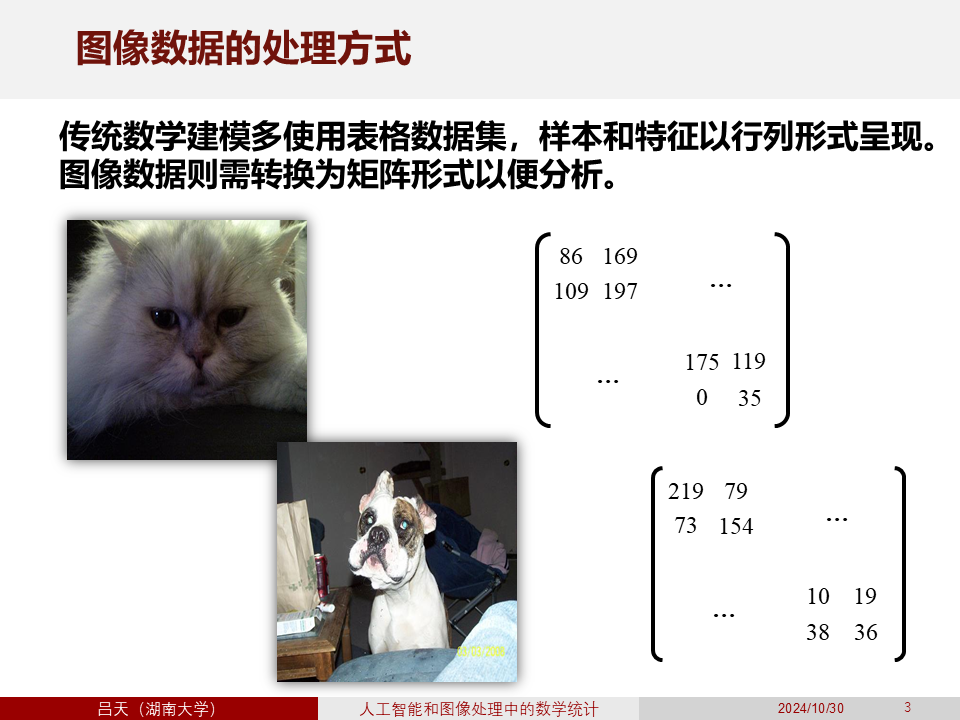
\includegraphics[width=\linewidth]{figures/图像数据的处理方式/1.PNG}
    \caption{图像数据的矩阵化表示}
\end{figure}
\vspace{-0.7em}

\section{RGB图像的分解与表示}

彩色图像可以看作由红、绿、蓝(RGB)三个颜色通道的矩阵叠加而成,每个通道对应一张灰度图。每个通道的数据均可表示为二维数组,其中每个元素的数值表示该像素在对应通道的强度。以 224×224×3 的彩色图像为例,该图像由三个 224×224 的二维矩阵构成,分别对应红、绿、蓝三种颜色通道。通过将RGB通道分解为独立的矩阵,能够对图像的颜色信息进行更为细致的分析。

\begin{figure}[H] % 图片位置固定
    \centering % 图片居中
    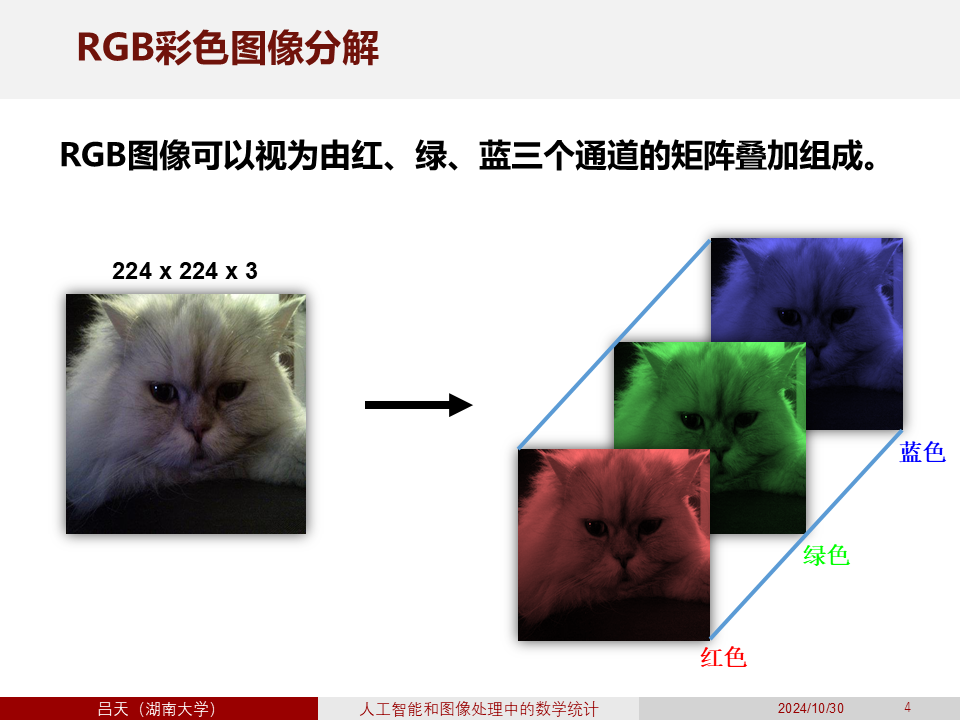
\includegraphics[width=\linewidth]{figures/图像数据的处理方式/2.PNG}
    \caption[RGB彩色图像的通道分解]{RGB彩色图像的通道分解。RGB图像可以分解为红、绿、蓝三个独立通道,每个通道都是一个灰度矩阵,表示对应颜色在图像中的强度分布。}
\end{figure}
\vspace{-0.7em}

\section{每个通道的数值结构}

在进一步处理RGB图像时,每个颜色通道的二维数组可以被视为一个独立的数值矩阵,这样的矩阵结构便于计算图像的统计特征。例如,对于图像矩的计算,我们可以分别计算红、绿、蓝三个通道的平均值、方差等统计量,从而获取图像的整体特征。这样的矩阵化表示使得图像分析方法可以与传统的数值统计方法相结合,为后续的图像处理与分类任务打下基础。

\begin{figure}[H] % 图片位置固定
    \centering % 图片居中
    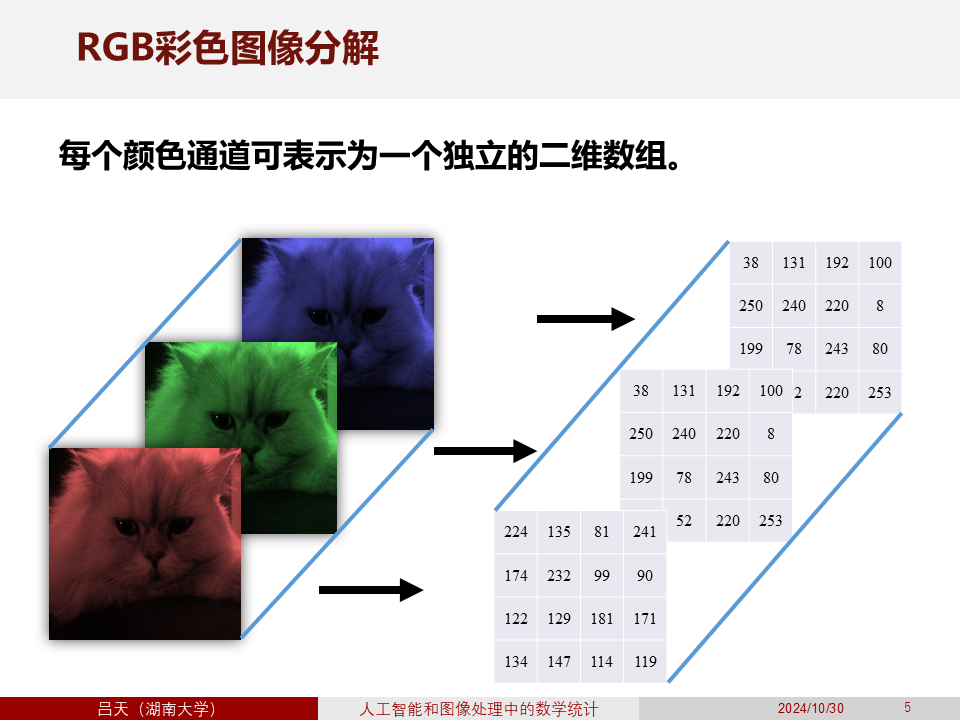
\includegraphics[width=\linewidth]{figures/图像数据的处理方式/3.PNG}
    \caption[每个颜色通道的矩阵表示]{每个颜色通道的矩阵表示。RGB图像的每个颜色通道可以表示为一个二维矩阵,每个元素值代表该通道下对应像素点的强度值。此表示方式便于计算图像的统计特征,如均值和方差。}
\end{figure}
\vspace{-0.7em}

\section{图像的样本矩}

样本矩是一种用于描述图像特征的方法,通过对像素灰度值的加权平均来衡量图像的特性或功能属性。样本矩分为原始矩和中心矩,用于不同的应用场景。

\subsection{原始矩}

原始矩用于描述图像的总体特征。定义如下:

\begin{equation}
M_{pq} = \sum_x \sum_y x^p y^q I(x, y)
\end{equation}

其中,\( I(x, y) \) 表示图像在位置 \( (x, y) \) 的灰度值,\( p \) 和 \( q \) 是非负整数,表示矩的阶数。

常用的原始矩包括:
\begin{itemize}
    \item \( M_{00} \):图像的零阶矩,对应图像的总灰度值。
    \item \( M_{10} \) 和 \( M_{01} \):用于计算图像的质心坐标。
\end{itemize}

\begin{figure}[H] % 图片位置固定
    \centering % 图片居中
    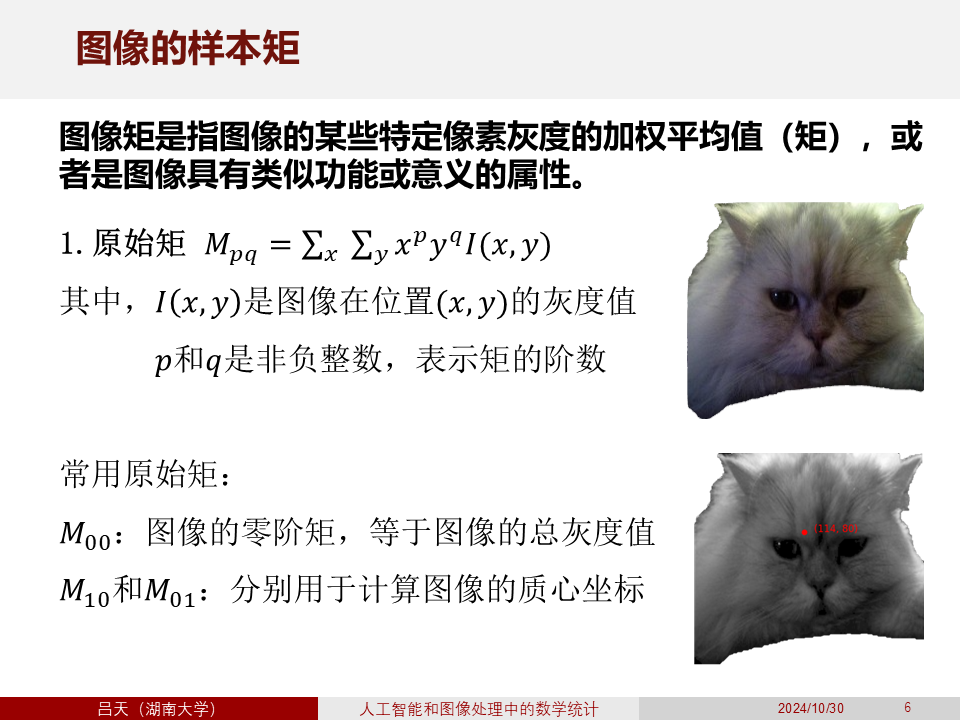
\includegraphics[width=\linewidth]{figures/图像数据的处理方式/4.PNG}
    \caption[图像的原始矩]{图像的原始矩。图像矩用于描述图像中某些特定像素灰度的加权平均值或功能属性,原始矩 $M_{pq}$ 表示为 $M_{pq} = \sum_x \sum_y x^p y^q I(x,y)$,其中 $I(x,y)$ 为像素灰度值,$p$ 和 $q$ 为非负整数。}
\end{figure}
\vspace{-0.7em}

\subsection{中心矩}

中心矩用于描述图像的形状特征,并对图像的平移不敏感。中心矩的定义如下:

\begin{equation}
\mu_{pq} = \sum_x \sum_y (x - \bar{x})^p (y - \bar{y})^q I(x, y)
\end{equation}

其中,\( \bar{x} \) 和 \( \bar{y} \) 表示图像的质心坐标。

常用的中心矩包括:
\begin{itemize}
    \item 二阶中心矩 \( \mu_{20}, \mu_{02}, \mu_{11} \),用于描述图像的方向性和散度。
\end{itemize}

\begin{figure}[H] % 图片位置固定
    \centering % 图片居中
    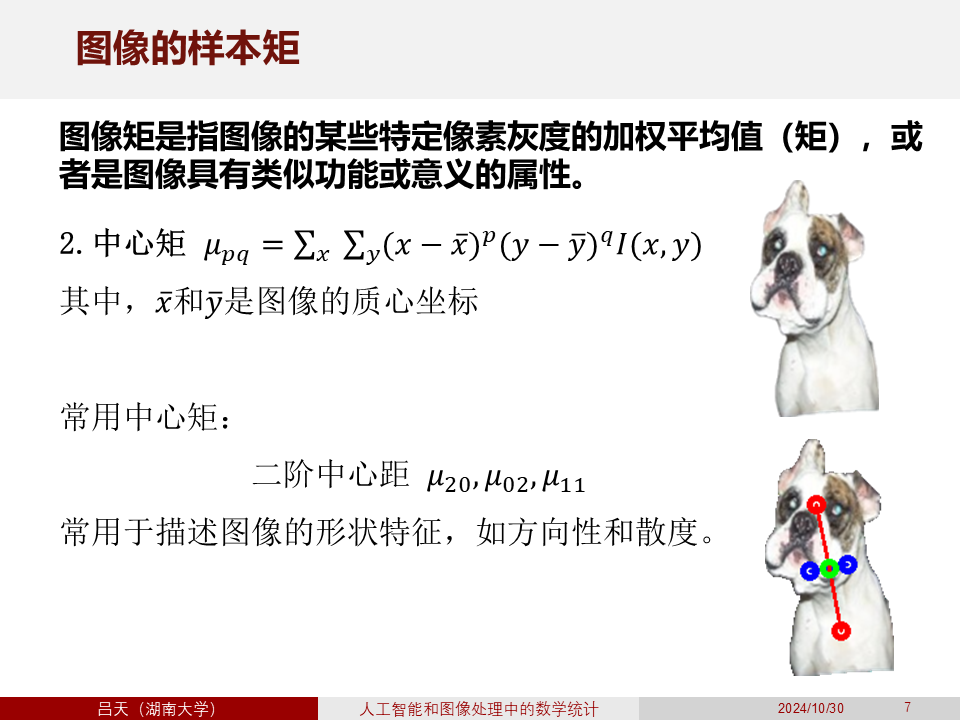
\includegraphics[width=\linewidth]{figures/图像数据的处理方式/5.PNG}
    \caption[图像的中心矩]{图像的中心矩。中心矩 $\mu_{pq}$ 表示为 $\mu_{pq} = \sum_x \sum_y (x - \bar{x})^p (y - \bar{y})^q I(x,y)$,其中 $\bar{x}$ 和 $\bar{y}$ 分别为图像的质心坐标,常用的中心矩如 $\mu_{20}$、$\mu_{02}$、$\mu_{11}$,通常用于描述图像的形状特征,如方向性和散度。}
\end{figure}
\vspace{-0.7em}

%%%%%%%%%%%%%%%%%%%%%%%%%%%%%%%%%%%%%%%%%%%%%%%%%%%%%%%%%%

\chapter{回归分析与梯度下降}

\section{一元线性回归的最小二乘拟合}

在回归分析中,一元线性回归是最基本的模型之一,适用于数据点沿线性趋势分布的情况。最小二乘法通过最小化数据点与拟合直线之间的误差平方和,来求得线性模型的最佳拟合参数。对于带有随机噪声的数据集,最小二乘法可以有效地拟合出近似的线性关系。

给定数据点集合 $\{(x_i, y_i)\}_{i=1}^n$,我们假设回归模型为:
\begin{equation}
    y = wx + b
\end{equation}
其中,$w$ 和 $b$ 分别为斜率和截距。最小二乘法的目标是找到使得误差平方和最小的 $w$ 和 $b$。因此,最小二乘损失函数定义为:
\begin{equation}
    L(w, b) = \sum_{i=1}^{n} (y_i - (wx_i + b))^2
\end{equation}
通过求解这个优化问题,我们可以获得最佳拟合的线性模型。

\begin{figure}[H]
    \centering
    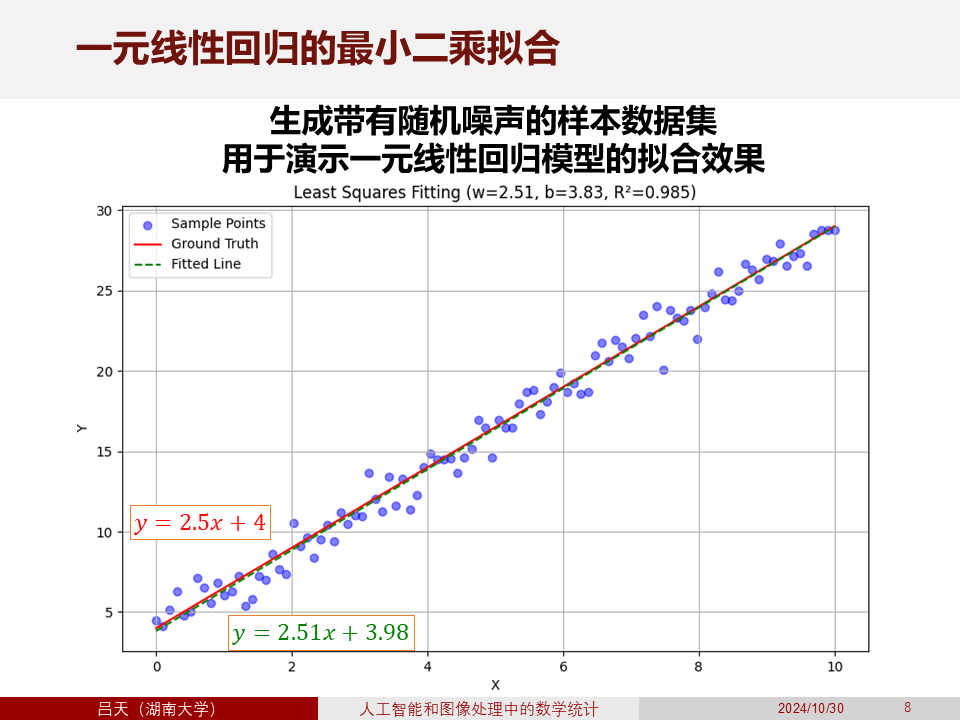
\includegraphics[width=\linewidth]{figures/回归分析与梯度下降/1.PNG}
    \caption{一元线性回归的最小二乘拟合}
    \label{fig:linear_least_squares}
\end{figure}

图\ref{fig:linear_least_squares} 展示了使用最小二乘法对随机噪声数据的拟合效果,绿色线表示拟合得到的直线,接近于真实的线性趋势。

\section{一元线性回归的梯度下降拟合}

在数据量较大时,直接求解最小二乘法的参数可能不具备计算效率。因此,我们可以采用梯度下降法来迭代更新参数,以逐步逼近最优解。梯度下降法通过计算损失函数对参数的偏导数来更新 $w$ 和 $b$ 的值。

梯度下降的参数更新公式为:
\begin{align}
    w &\leftarrow w - \alpha \frac{\partial L(w, b)}{\partial w} \\
    b &\leftarrow b - \alpha \frac{\partial L(w, b)}{\partial b}
\end{align}
其中,$\alpha$ 为学习率,控制每次更新的步长大小。通过多次迭代更新参数,最终可以得到拟合优良的直线。

\begin{figure}[H]
    \centering
    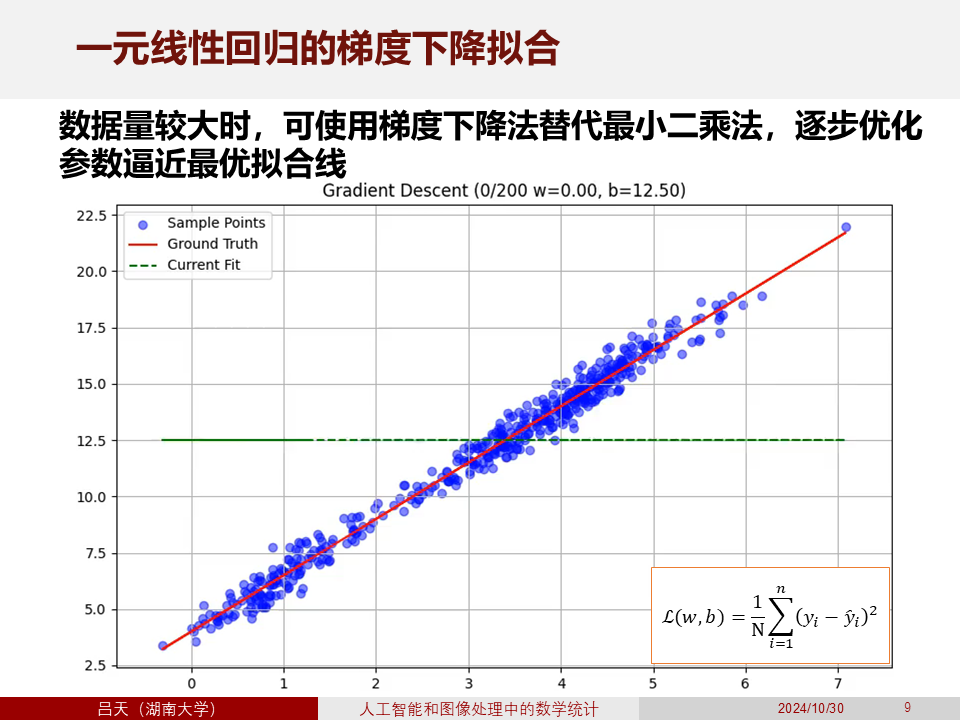
\includegraphics[width=\linewidth]{figures/回归分析与梯度下降/2.PNG}
    \caption[一元线性回归的梯度下降拟合]{一元线性回归的梯度下降拟合。视频在\href{https://github.com/PhD-TianLv/Mathematical-Statistics-in-Artificial-Intelligence-and-Image-Processing/blob/main/videos/1-一元线性回归的梯度下降拟合.mp4}{GitHub}\footnotemark 中可见。}
    \label{fig:linear_gradient_descent}
\end{figure}

\footnotetext{https://github.com/PhD-TianLv/Mathematical-Statistics-in-Artificial-Intelligence-and-Image-Processing/blob/main/videos/1-一元线性回归的梯度下降拟合.mp4}

图\ref{fig:linear_gradient_descent} 展示了使用梯度下降法对同样数据集的拟合过程,通过逐步更新参数,拟合线逐渐逼近真实的线性趋势。

\section{非线性回归与神经网络拟合}

当数据呈现复杂的非线性特征时,如螺旋曲线,一元或多项式回归难以精确拟合。此时,神经网络可以作为通用拟合器,通过学习复杂的非线性映射关系,实现对数据的精确拟合。

我们使用神经网络构建非线性模型,通过优化损失函数来调整神经网络的参数。神经网络的损失函数可定义为:
\begin{equation}
    L(\theta) = \frac{1}{N} \sum_{i=1}^{N} \left[ (x_i - \hat{x}(t_i; \theta))^2 + (y_i - \hat{y}(t_i; \theta))^2 \right]
\end{equation}
其中,$\theta$ 为神经网络的参数,通过反向传播算法和梯度下降方法更新,以最小化损失函数,实现精确的曲线拟合。

\begin{figure}[H]
    \centering
    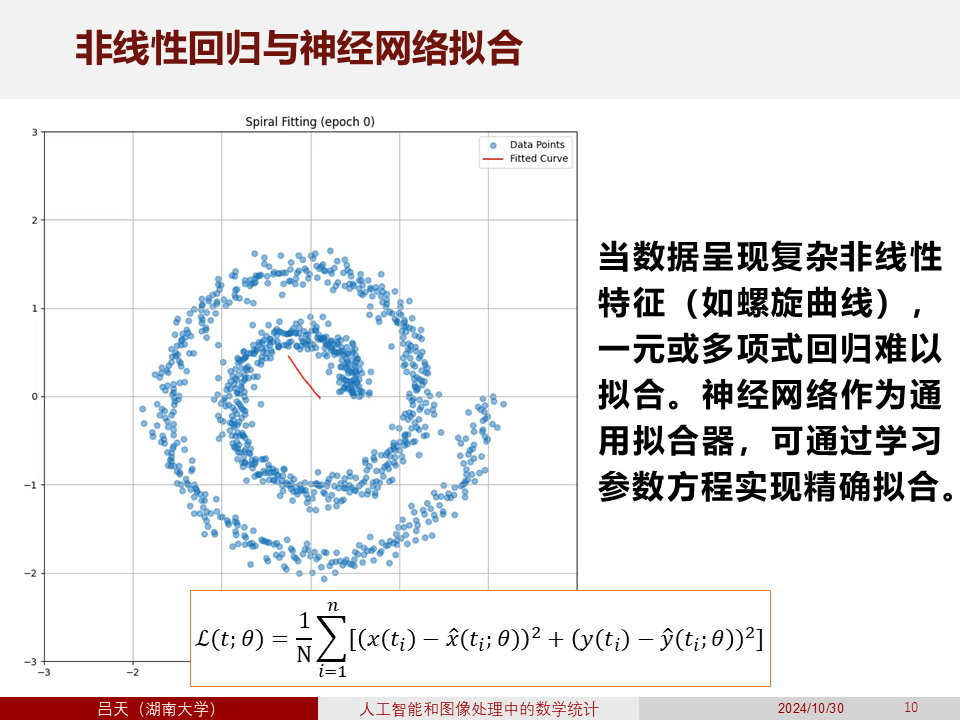
\includegraphics[width=\linewidth]{figures/回归分析与梯度下降/3.PNG}
    \caption[非线性回归与神经网络拟合]{非线性回归与神经网络拟合。视频在\href{https://github.com/PhD-TianLv/Mathematical-Statistics-in-Artificial-Intelligence-and-Image-Processing/blob/main/videos/2-非线性回归与神经网络拟合.mp4}{Github}\footnotemark 中可见。}
    \label{fig:nonlinear_regression_nn}
\end{figure}

\footnotetext{https://github.com/PhD-TianLv/Mathematical-Statistics-in-Artificial-Intelligence-and-Image-Processing/blob/main/videos/2-非线性回归与神经网络拟合.mp4}

图\ref{fig:nonlinear_regression_nn} 中展示了神经网络对螺旋形数据的拟合效果。由于神经网络能够学习复杂的非线性关系,其拟合效果显著优于线性回归。

%%%%%%%%%%%%%%%%%%%%%%%%%%%%%%%%%%%%%%%%%%%%%%%%%%%%%%%%%%

\chapter{神经网络分类的原理与实现}

\section{分类的本质:映射到可分离的特征空间}

在分类任务中,目标是找到一个能够有效区分不同类别的特征空间。通过将数据映射到高维特征空间,可以使原本难以分离的样本实现线性分离。例如,在图像分类中,二维空间中的复杂数据(如螺旋形数据)可以通过添加第三维来实现清晰的分离。在三维空间中,不同类别可以通过 z 轴位置进行区分。

\begin{figure}[H]
    \centering
    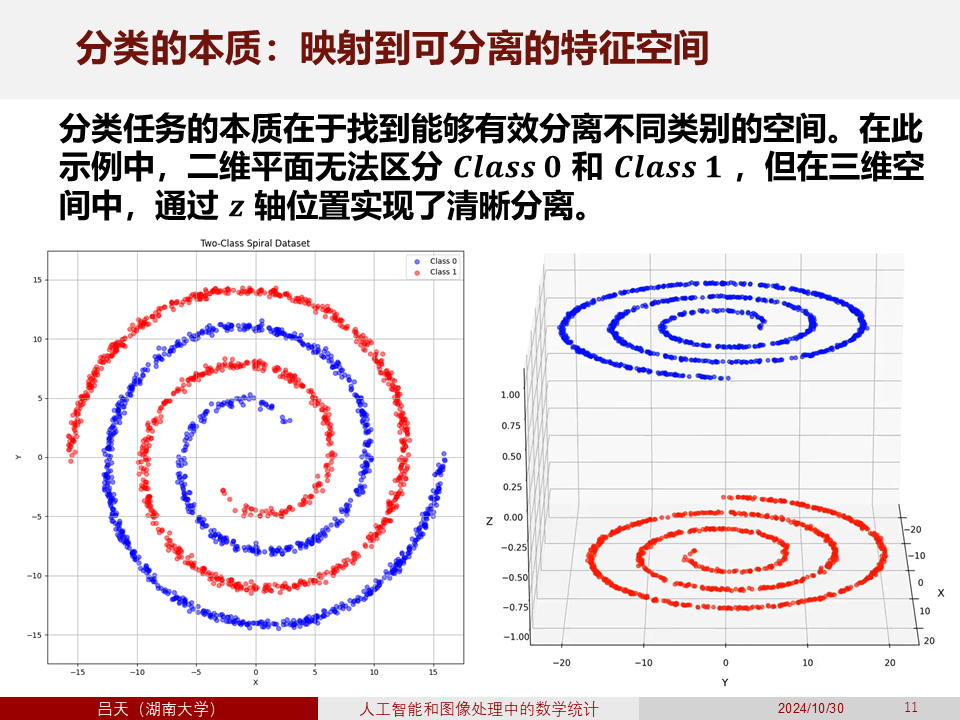
\includegraphics[width=\linewidth]{figures/神经网络分类的原理与实现/1.PNG}
    \caption[通过将数据映射到高维空间实现清晰分离]{通过将数据映射到高维空间实现清晰分离。视频在\href{https://github.com/PhD-TianLv/Mathematical-Statistics-in-Artificial-Intelligence-and-Image-Processing/blob/main/videos/3-分类的本质:映射到可分离的特征空间.mp4}{Github}\footnotemark 中可见。}
\end{figure}

\footnotetext{https://github.com/PhD-TianLv/Mathematical-Statistics-in-Artificial-Intelligence-and-Image-Processing/blob/main/videos/3-分类的本质:映射到可分离的特征空间.mp4}

\section{神经网络的分类过程}

神经网络能够通过将输入数据转换为特征向量,实现不同类别在特征空间中的分离。这一过程主要通过多个层次的非线性变换,使得同一类数据在特征空间中聚集,而不同类的数据彼此分离。最终,分类边界通过神经网络的决策边界形成,区分不同类别。

\begin{figure}[H]
    \centering
    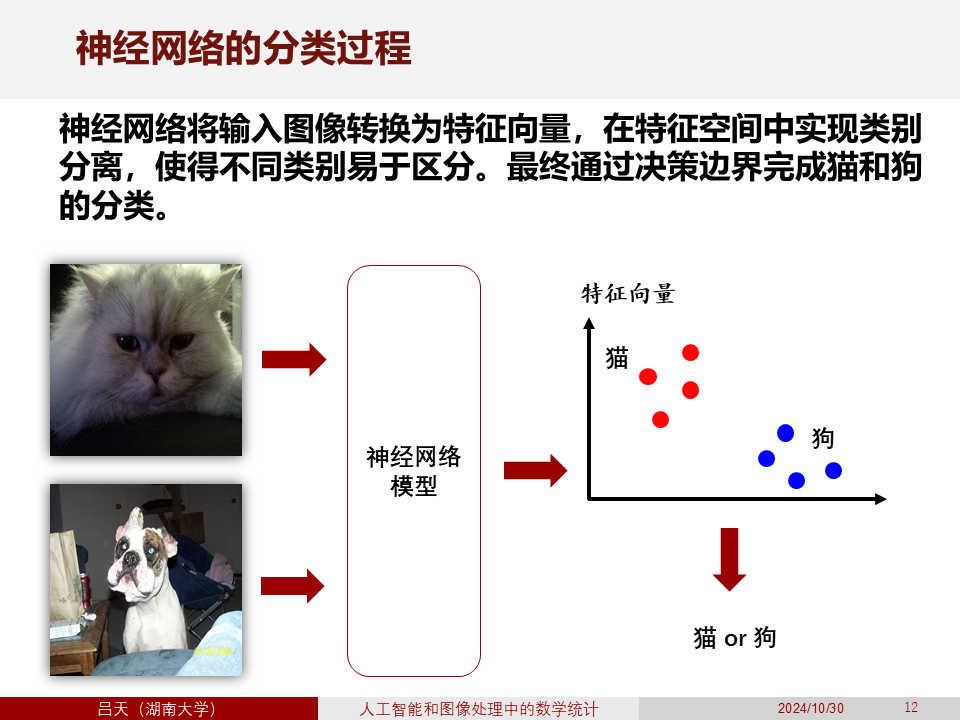
\includegraphics[width=\linewidth]{figures/神经网络分类的原理与实现/2.PNG}
    \caption{神经网络通过特征变换完成分类任务}
\end{figure}

\section{基于极大似然估计的分类损失函数求解}

在分类任务中,极大似然估计是一种常用的优化方法,用于最小化预测概率分布与真实分布之间的差异。设 \(\mathbf{Y} | \mathbf{X}\) 为输出数据的条件概率分布,则其联合概率可以表示为:

\begin{equation}
P(\mathbf{Y}|\mathbf{X}) = \prod_{i=1}^n P(y^{(i)}|\mathbf{x}^{(i)})
\end{equation}

对数似然函数定义为:

\begin{equation}
- \log P(\mathbf{Y}|\mathbf{X}) = \sum_{i=1}^n - \log P(y^{(i)}|\mathbf{x}^{(i)})
\end{equation}

\section{交叉熵损失函数}

交叉熵损失函数是用于衡量分类模型输出分布与真实分布之间差异的常用损失函数。定义为:

\begin{equation}
L(\mathbf{y}, \hat{\mathbf{y}}) = - \sum_{j=1}^q y_j \log \hat{y}_j
\end{equation}

其中,\( q \) 是类别数,\( y \) 是真实标签的独热编码,\( \hat{y} \) 是模型预测的概率分布。

\begin{figure}[H]
    \centering
    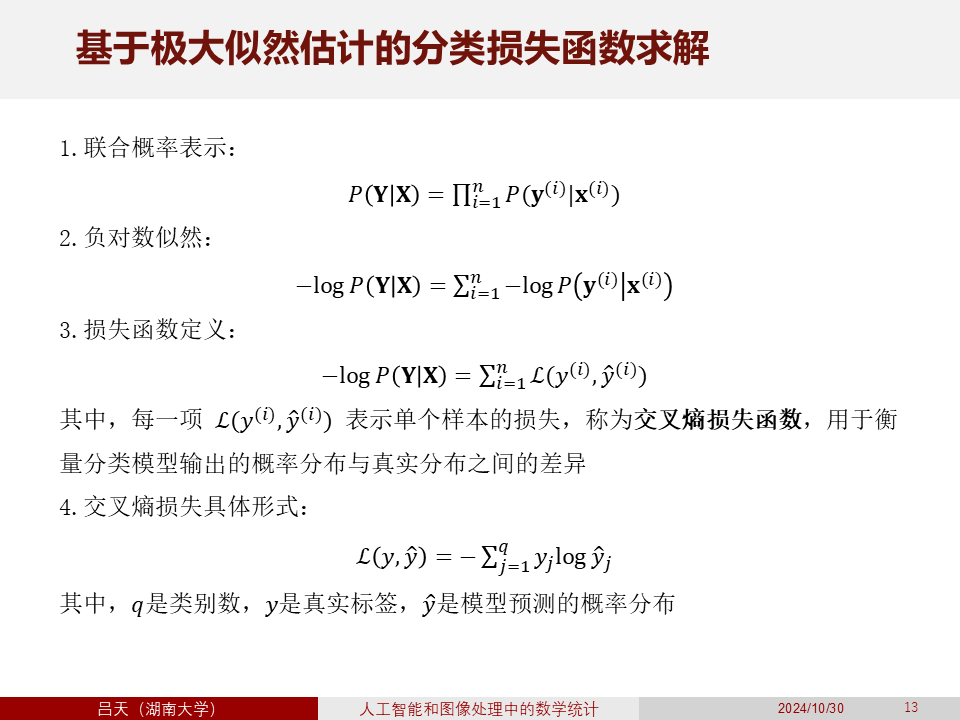
\includegraphics[width=\linewidth]{figures/神经网络分类的原理与实现/3.PNG}
    \caption{基于极大似然估计的分类损失函数求解过程}
\end{figure}

%%%%%%%%%%%%%%%%%%%%%%%%%%%%%%%%%%%%%%%%%%%%%%%%%%%%%%%%%%

\chapter{基于对比学习的跨模态分类}

\section{对比学习概述}

对比学习(Contrastive Learning)是一种通过比较样本之间相似性来学习特征表示的方法。在对比学习的框架中,模型被训练以将相似的样本映射到特征空间中靠近的位置,而将不相似的样本映射到远离的位置。这种方法在图像和文本等不同模态数据的处理上表现出色,尤其适用于跨模态任务中的分类。

\section{CLIP模型的跨模态映射}

CLIP\cite{clip} (Contrastive Language-Image Pretraining) 模型是一种能够将图像和文本映射到同一特征空间的模型。通过对图像和文本的联合训练,CLIP 模型可以在同一特征空间中将相似的图像-文本对拉近,同时将不相关的对拉远,从而实现跨模态的对比学习。其核心原理如下:

\begin{itemize}
    \item 将图像和文本分别通过特定的神经网络模型(如 ResNet\cite{resnet} 和 Transformer\cite{ViT})提取特征。
    \item 将提取的特征映射到同一向量空间中,并通过对比损失函数来优化特征,使得相似对在特征空间中靠近,不相似对则距离较远。
\end{itemize}

\section{CLIP模型在真实图像与AI生成图像分类中的应用}

利用 CLIP 模型的跨模态特征对比能力,可以有效区分真实图像和 AI 生成的图像\cite{universalfakedetect}。CLIP 模型能够将真实图像和 AI 生成图像映射到同一特征空间中,通过计算其特征向量的相似度来判断图像的来源。具体实现方法包括:

\begin{itemize}
    \item 输入真实图像和 AI 生成图像,通过 CLIP 模型得到对应的特征向量。
    \item 通过计算不同图像特征向量之间的距离,确定图像的类别,从而实现更为精确的分类效果。
\end{itemize}

\begin{figure}[H]
    \centering
    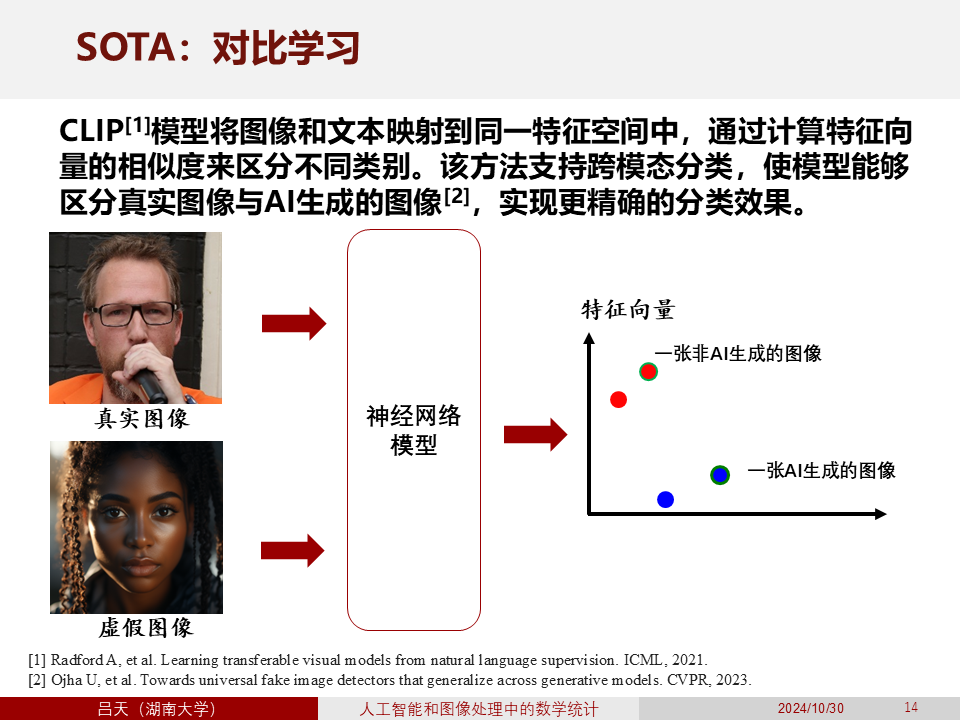
\includegraphics[width=\linewidth]{figures/基于对比学习的跨模态分类/1.PNG}
    \caption{CLIP 模型的跨模态特征映射与分类过程}
\end{figure}

%%%%%%%%%%%%%%%%%%%%%%%%%%%%%%%%%%%%%%%%%%%%%%%%%%%%%%%%%%

\chapter{总结}

本论文系统性地探讨了数学统计方法在人工智能与图像处理中的应用,涵盖了从传统回归分析到现代神经网络与对比学习的跨模态分类方法。首先,论文介绍了图像数据的矩阵化表示及其各通道的特征分解,为后续的数据处理奠定了基础。通过对图像矩的分析,展示了如何利用统计矩描述图像的几何属性和灰度分布特性,为图像特征提取提供了理论支持。

在回归分析部分,论文深入比较了一元线性回归的最小二乘拟合与梯度下降法,并引入了非线性回归与神经网络拟合的应用,以解决传统回归方法在处理复杂数据特征上的局限。此部分表明,神经网络的自适应非线性映射能力,使其成为拟合复杂非线性数据的理想工具。

分类任务中,通过分析神经网络模型在高维特征空间中的映射和分离机制,阐述了神经网络在特征空间中实现有效分类的原理。同时,论文对基于极大似然估计的分类损失函数进行了详细推导,并探讨了交叉熵损失在优化分类模型性能上的优势。

在跨模态分类的应用上,论文最后引入了CLIP模型,展示了其在多模态数据(图像与文本)处理中的优越性。CLIP模型通过对比学习将不同模态的输入映射到同一特征空间,从而实现准确的跨模态分类能力,进一步提升了分类模型的应用范围与准确度。

综上所述,本研究通过将数学统计与深度学习相结合,为图像处理与智能分类提供了高效的理论框架和实践参考,展示了数学统计方法在人工智能与图像处理中的重要价值。

%%%%%%%%%%%%%%%%%%%%%%%%%%%%%%%%%%%%%%%%%%%%%%%%%%%%%%%%%%




%%%%%%%%%%%%%%%%%%%%%%%%  参考文献  %%%%%%%%%%%%%%%%%%%%%%%%

\begin{references}
    \bibliography{references.bib} % 指定.bib文件路径
\end{references}

%%%%%%%%%%%%%%%%%%%%%%%%%  附录  %%%%%%%%%%%%%%%%%%%%%%%%%%

% \StartAppendix % 启用附录

% \chapter{附录}

% 附录

%%%%%%%%%%%%%%%%%%%%%%%  正文后页眉  %%%%%%%%%%%%%%%%%%%%%%

% 页眉(关闭页眉务必将页眉类型设为empty)
\Header
    {common} % 页眉类型:common、publish、empty
    {1pt} % 上分隔线宽度
    {1pt} % 两线距离
    {0.5pt} % 下分割线宽度
    {} % 页眉左自定义内容(文本或图片)
    {
\includegraphics[width=0.25\textwidth]{figures/logos/HNU-title-EN.png}} % 页眉中自定义内容(文本或图片)
    {} % 页眉右自定义内容(文本或图片)

%============================================%

% 页脚(关闭页脚务必将页脚类型设为empty) 
\Footer
    {common} % 页脚类型:common、publish、empty
    {0pt} % 上分隔线宽度
    {0pt} % 两线距离
    {0pt} % 下分割线宽度
    {} % 页脚左自定义内容(文本或图片)
    {\thepage} % 页脚中自定义内容(文本或图片)
    {} % 页脚右自定义内容(文本或图片)

%============================================%

% 页数样式 参数:#1起始页数
% \setRomanPageNumber{1} % 设置罗马数字页码
% \setArabicPageNumber{1} % 设置阿拉伯数字页码

%%%%%%%%%%%%%%%%%%%%%%%%%  致谢  %%%%%%%%%%%%%%%%%%%%%%%%%

% \StartAcknowledgements % 启用致谢

\end{document}